\documentclass{article}
\usepackage[screen]{geometry}
\usepackage{alltt,xcolor}
\usepackage[utf8]{inputenc}
\usepackage{listings}
\usepackage{graphicx}

\lstset{escapechar=\@,language=C++,keywordstyle=\color{blue},showstringspaces=false}
\begin{document}
	
\section*{Specification}
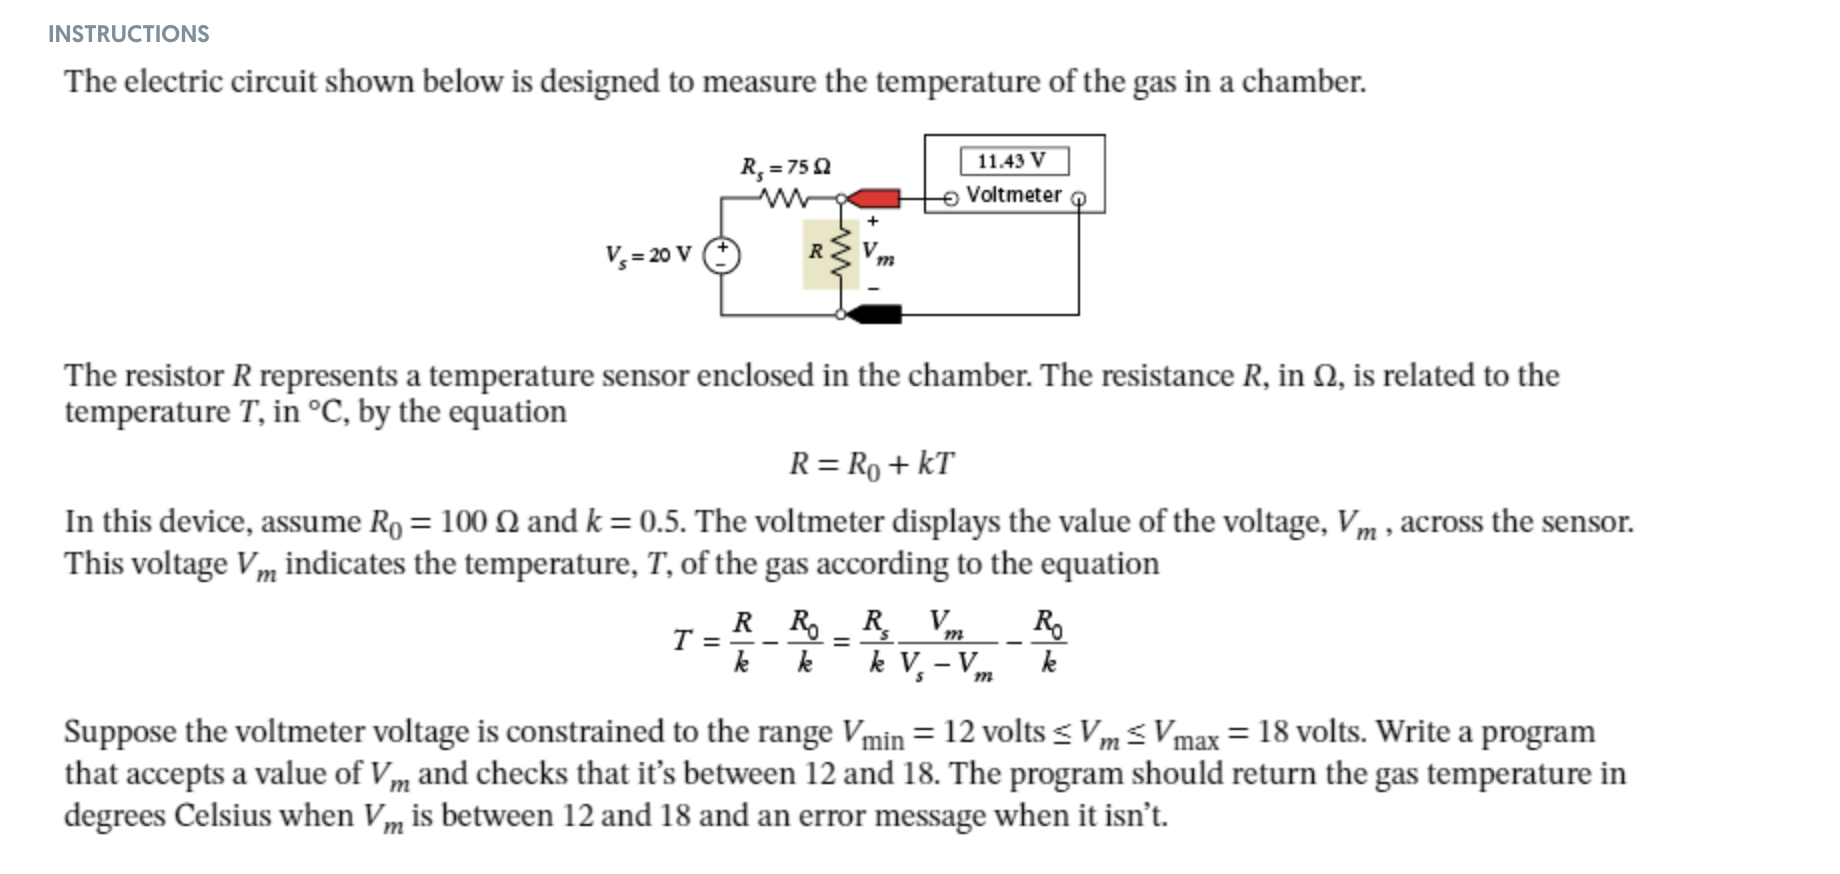
\includegraphics[scale=0.7]{lab2.png}
\begin{description}
	\item The programe will show a window to the users and tell them to enter the voltage and then output the gas temperature as the question tells us.
\end{description}


\newpage\section*{Analysis}
\begin{description}
	\item [Inputs]  The voltage $V_{m},R_{0} = 100 \Omega, k = 0.5,R_{s} = 75 \; \Omega, V_{s} = 20 V $
	\item [Process]  Calculate temperature T from input $V_{m}$
	where \[ T =\frac{R_{s}}{k} \times \frac{V_{m}}{V_{s - V_{m}}}
	   - \frac{R_{0}}{k} \]
	   where $R_{0} = 100 \Omega, k = 0.5,R_{s} = 75 \; \Omega, V_{s} = 20 V $
    \item [Outputs]  The temperature in Celsius or error message
\end{description}

\newpage\section*{Design}

\begin{itemize}
	\item Create constants for the question.
	$R_{0} = 100 \Omega, k = 0.5,R_{s} = 75 \; \Omega, V_{s} = 20 V $
	\item As the question tells us,we should use the equation, which is shown .So we should use the following equation in our programe to calculate the gas temperature.
	$T= \frac{Rs*Vm}{k*(Vs-Vm)}-\frac{R0}{k}$ 
	\item What's more,we should test if the user typed a wrong thing in our software.
	\item So in this case,our code will be execute successfully.
\end{itemize}
\newpage\section*{Implementation}
\lstinputlisting{lab.cpp}
\lstinputlisting{labgui.cpp}
\lstinputlisting{labgui.h}
\newpage\section*{Test}
\subsection*{Testcase 1}
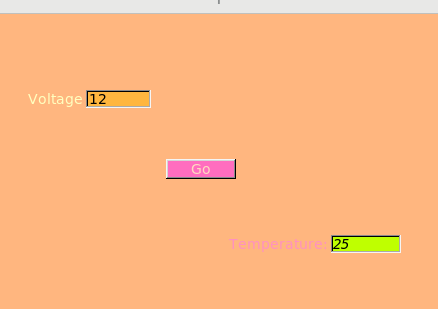
\includegraphics{testcase1.png}
\begin{itemize}
	\item So when our input is 12,our output must be 25,which is exactly correct.
	\item like $25= \frac{75*12}{0.5*(20-12)}-\frac{100}{0.5}$ 
	\item Since our output is exactly 25,our testcase1 is passed.
\end{itemize}
\subsection*{Testcase 2}
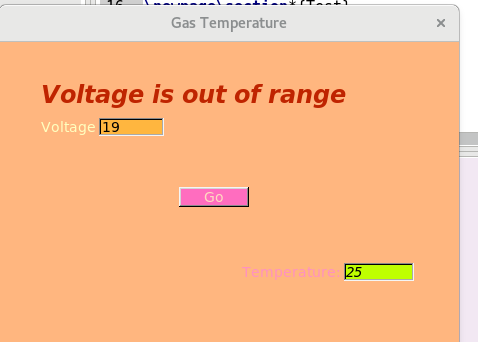
\includegraphics{testcase2.png}
\begin{itemize}
	\item So when our input is 19,our output must be the message that tells user the voltage is out of range.
	\item Since our output is exactly what we need as the picture shows,our testcase2 is passed.
\end{itemize}
\end{document}
